\documentclass[10pt,a4paper]{article}
\usepackage[margin=1.5cm]{geometry}
\usepackage{amsmath,amssymb}
\usepackage{graphicx}
\usepackage{booktabs}
\usepackage{caption}
\usepackage[colorlinks=true,linkcolor=blue,citecolor=blue,urlcolor=blue]{hyperref}
\usepackage[numbers,sort&compress]{natbib}
\usepackage{microtype}
\captionsetup{font=small,labelfont=bf}
\setlength{\parskip}{1pt}
\setlength{\textfloatsep}{6pt}
\setlength{\floatsep}{6pt}
\setlength{\abovecaptionskip}{3pt}
\newcommand{\ClMAEpct}{5.1}
\newcommand{\ClMaeLadson}{0.0379}
\newcommand{\ClMaeAbbott}{0.0581}
\newcommand{\ClMaeGregory}{0.0548}
\newcommand{\CdMaeLadsonAbs}{0.0099}
\newcommand{\CflThreeDClPct}{10.3}
\newcommand{\CflThreeDClFifteen}{-34}
\newcommand{\CpMaeZero}{0.019}
\newcommand{\CpMaeTen}{0.119}
\newcommand{\CpMaeFifteen}{0.688}
\newcommand{\ClZeroZeroOneTwoZero}{0.0062}
\newcommand{\SepAten}{$>0.99$ (attached)}
\newcommand{\SepAfifteen}{0.20}
\newcommand{\LdMaxZeroZeroOneTwo}{35.9}
\newcommand{\LdMaxFourFourOneTwo}{39.8}
\newcommand{\NumCoarse}{16{,}100}
\newcommand{\NumMedium}{33{,}740}
\newcommand{\NumFine}{51{,}360}
\newcommand{\ClCoarse}{0.5074}
\newcommand{\ClMedium}{0.5280}
\newcommand{\ClFine}{0.5311}
\newcommand{\ClGridDelta}{0.58\%}
\newcommand{\CdGridDelta}{0.05\%}
\newcommand{\SepTableRows}{0 & 0.0062 & 0.0142 & 0.4 & $>0.99$ (attached) \\
    10 & 0.9663 & 0.0269 & 35.9 & $>0.99$ (attached) \\
    15 & 0.9915 & 0.0928 & 10.7 & 0.20 \\
    18 & 1.0175 & 0.1333 & 7.6 & 0.17 \\
    5 & 0.5280 & 0.0171 & 30.9 & $>0.99$ (attached) \\}
\newcommand{\ReTableRows}{$10^5$ & 0.9062 & 0.0395 & 22.9 & 0.03 \\
    $3\times10^5$ & 0.9345 & 0.0320 & 29.2 & $>0.99$ (attached) \\
    $10^6$ & 0.9663 & 0.0269 & 35.9 & $>0.99$ (attached) \\}
\newcommand{\ReClDropPct}{6}
\newcommand{\ReCdRisePct}{47}
\newcommand{\ReClDropThreePct}{3}
\newcommand{\ReCdRiseThreePct}{19}
\newcommand{\SepReLow}{0.03}
\newcommand{\LdReSix}{35.9}
\newcommand{\LdReFive}{22.9}
\newcommand{\GridHighRows}{Medium & 4000 iters & 0.9663 & 0.0269 \\
    Fine & 4000 iters & 0.9724 & 0.0271 \\
    Medium & 12000 iters & 0.9552 & 0.0268 \\
    Medium, $R=50c$ & 4000 iters & 0.9403 & 0.0273 \\}
\newcommand{\SerrTableRows}{5 & 0.5280 & 0.4991 & 0.0171 & 0.0186 \\
    10 & 0.9663 & 0.9642 & 0.0269 & 0.0294 \\
    15 & 0.9915 & 1.1398 & 0.0928 & 0.0802 \\}
\newcommand{\SerrCdDropFive}{-8.6}
\newcommand{\SerrClDropFive}{5.5}
\newcommand{\SerrCdDropFifteen}{13.6}
\newcommand{\SerrClRiseFifteen}{15.0}
\newcommand{\SerrCdIncrFive}{8.6}
\newcommand{\AllForcesRows}{NACA0012 & 0 & 0.0062 & 0.0142 & 0.4 \\
    NACA0012 & 10 & 0.9663 & 0.0269 & 35.9 \\
    NACA0012 & 15 & 0.9915 & 0.0928 & 10.7 \\
    NACA0012 & 18 & 1.0175 & 0.1333 & 7.6 \\
    NACA0012 & 5 & 0.5280 & 0.0171 & 30.9 \\
    NACA2412 & 0 & 0.2048 & 0.0155 & 13.2 \\
    NACA2412 & 10 & 1.1255 & 0.0307 & 36.6 \\
    NACA2412 & 15 & 1.2910 & 0.0671 & 19.3 \\
    NACA2412 & 18 & 1.3513 & 0.0995 & 13.6 \\
    NACA2412 & 5 & 0.7039 & 0.0196 & 35.9 \\
    NACA4412 & 0 & 0.3980 & 0.0168 & 23.7 \\
    NACA4412 & 10 & 1.2877 & 0.0339 & 38.0 \\
    NACA4412 & 15 & 1.4757 & 0.0655 & 22.5 \\
    NACA4412 & 18 & 1.4138 & 0.1108 & 12.8 \\
    NACA4412 & 5 & 0.8835 & 0.0222 & 39.8 \\}
\newcommand{\NonOrthCoarse}{81.9667}
\newcommand{\NonOrthAvgCoarse}{37.91366}
\newcommand{\SkewCoarse}{3.300121}
\newcommand{\NonOrthMedium}{82.67556}
\newcommand{\NonOrthAvgMedium}{41.93826}
\newcommand{\SkewMedium}{2.787854}
\newcommand{\NonOrthFine}{86.24867}
\newcommand{\NonOrthAvgFine}{42.8548}
\newcommand{\SkewFine}{2.008822}
\newcommand{\GciPct}{1}


\title{\textbf{Transition-Sensitive RANS Modelling of Boundary-Layer Separation on NACA 4-Digit Airfoils:\\ A Validated 2D Study (Extended Abstract)}}
\author{Md Mushfiqur Rahim\\
  \small ORCID: 0009-0003-1021-685X \quad Independent Researcher\\
  \small AERO-BLS Project --- OpenFOAM v2412 / $k$--$\omega$ SST / $Re=10^5$--$10^6$}
\date{\today}

\begin{document}
\maketitle
\vspace{-1.6em}

\begin{abstract}
\noindent Two-dimensional RANS simulations (125 runs: 123 steady + 2 URANS) characterise boundary-layer separation, stall, and transition-sensitive drag on the NACA 0012, 2412, and 4412 sections at $Re = 10^5$--$10^6$, $\alpha = 0^\circ$--$20^\circ$, using OpenFOAM on structured polar O-grids ($y^+ \approx 0.4$). Against the Reynolds-matched Sandia SAND80-2114 free-transition data, the $\gamma$--$Re_{\theta t}$ closure cuts the pre-stall drag mean absolute error by \SandiaCdErrDropPct{}~\% (to \SandiaCdMaeTR) relative to fully turbulent $k$--$\omega$ SST, and produces laminar separation bubbles the fully turbulent closure cannot generate. Steady separation onset at stall is shown to be grid-branch-dependent (three grids, three branches at $\alpha = 15^\circ$), while post-stall grids agree ($\alpha = 18^\circ$: same branch, drag within 3\%). A doubled-horizon URANS verification ($t^* = 0.81$--$2.4$, $n = 61$) shows the converged steady state is not an attractor of the time-accurate system, and the steady and URANS mean drags bracket the experiment. 2D surrogates of serrations and tubercles are reported as an explicit negative control. All meshes, cases, scripts, and figures are released for full reproducibility.
\end{abstract}

\section{Method}
\vspace{-0.4em}
The governing equations are the incompressible RANS equations closed with the $k$--$\omega$ SST model, and, in a 45-case factorial block, the four-equation $\gamma$--$Re_{\theta t}$ correlation-based transition model of Langtry and Menter~\cite{langtry2009}. Sections are generated analytically (638 points, cosine clustering) and meshed with Gmsh into polar O-grids (medium: 33{,}740 cells; fine: 51{,}360; $y^+ \approx 0.4$; farfield 20 chords, 50 chords for verification). The case matrix comprises: a three-airfoil core at $Re = 10^6$ (21 cases); a two-Reynolds sweep (30); grid families at $\alpha = 5^\circ$, $15^\circ$, and a fine repeat at $18^\circ$ (5); passive-device surrogates (8); the transition factorial (45); a Reynolds-matched low-$Re$ validation set (10); verification repeats (4); and two URANS cases (\texttt{pimpleFoam}, $\alpha = 12^\circ/15^\circ$, $Re = 3.6\times10^5$). Steady cases run 4{,}000 iterations with averaged forces over the final window; separation points are extracted from wall skin-friction reversal.

\section{Results}
\vspace{-0.4em}

\textbf{Validation.} On the NACA 0012 at $Re = 10^6$ the computed attached-range lift matches the tripped Ladson data to \ClMAEpct{}~\% MAE, and the setup reproduces the NASA CFL3D SST reference to within a few percent (code verification). Against the Reynolds-matched, free-transition Sandia data ($Re = 3.6\times10^5$; Fig.~\ref{fig:sandia}), the transition closure cuts the pre-stall drag MAE by \SandiaCdErrDropPct{}~\% (to \SandiaCdMaeTR) by recovering the laminar run. Neither closure reproduces the measured bubble-burst stall ($C_{L,\max}$ at $\alpha = 10^\circ$): the modelled stall angle at $Re \lesssim 4\times10^5$ is an upper bound.

\textbf{Separation and stall.} The separation-point map spans $x/c = 0.06$--$0.75$ (laminar bubbles) and the fully turbulent attached-to-separated transition across all three sections; camber delays upper-surface separation and raises $C_{L,\max}$ monotonically from 0012 to 4412. Reducing $Re$ from $10^6$ to $10^5$ shifts separation forward and degrades $C_L/C_D$ substantially on all sections.

\textbf{Grid sensitivity as branch selection.} At the stall angle $\alpha = 15^\circ$ the three grids select three different separation branches ($x/c = 0.53$ coarse, $0.20$ medium, attached fine), so no global grid-converged answer exists there; attached-flow grid sensitivity is \ClGridDelta{}~\% in $C_L$ and \CdGridDelta{}~\% in $C_D$ ($\alpha = 5^\circ$). At the post-stall angle $\alpha = 18^\circ$, medium and fine grids select the \emph{same} deeply separated branch (separation $x/c = 0.17$ vs $0.15$, drag within 3\%), confining the grid sensitivity to the stall-onset angle.

\textbf{URANS: the steady state is not an attractor.} A doubled-horizon URANS verification ($t = 0.15$--$0.45$~s, $t^* = 0.81$--$2.4$, 61 samples; Fig.~\ref{fig:urans}) shows genuinely unsteady loads (drag std 24--41\% of the mean) and time means that do not recover the steady solution: mean lift exceeds the steady value by 27\% ($\alpha = 12^\circ$: $1.322 \pm 0.068$ vs $1.039$) and 34\% ($\alpha = 15^\circ$: $1.415 \pm 0.108$ vs $1.058$), still drifting at the end of the window. At $\alpha = 15^\circ$ the steady ($0.075$) and URANS ($0.307$) mean drags bracket the measured value ($0.190$) --- horizon-averaged loads of this non-stationary system depend on the window.

\textbf{2D devices are a negative control.} Serrated-trailing-edge and leading-edge-tubercle surrogates \emph{increase} drag (up to \TubCdPctTen{}~\% for the tubercle at $\alpha = 10^\circ$) where 3D experiments show gains: both devices operate through spanwise mechanisms a 2D model cannot represent. The computations quantify the screening error of dimensionality-mismatched device models rather than device performance.

\begin{figure}[t]
  \centering
  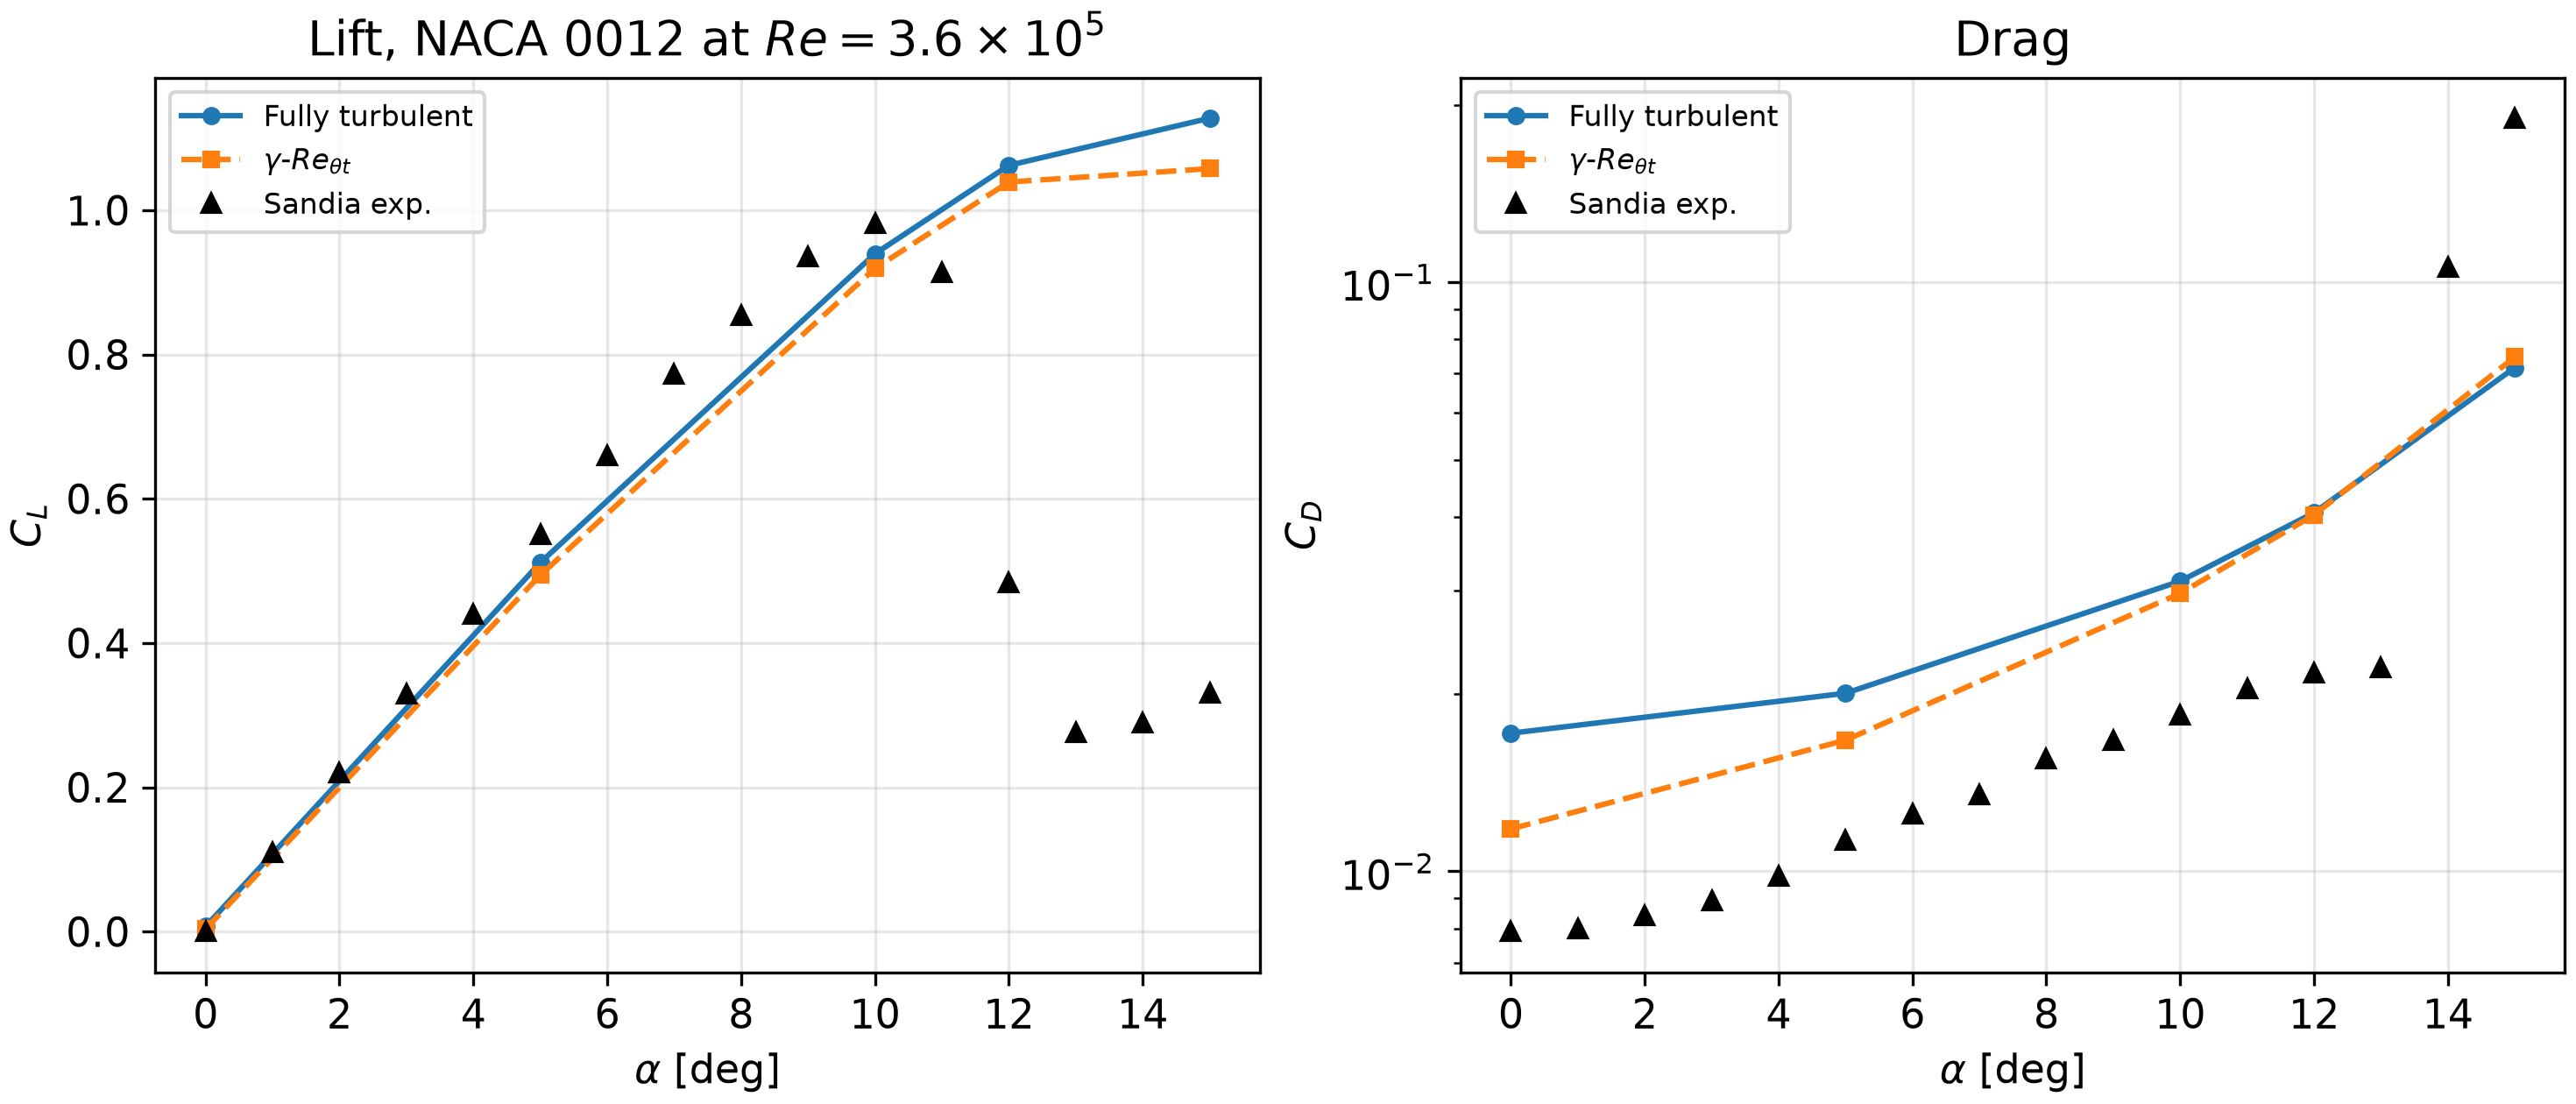
\includegraphics[width=0.72\textwidth]{figures/fig14_sandia_validation.png}
  \caption{Reynolds-matched validation: NACA 0012 at $Re = 3.6\times10^5$ against the free-transition Sandia data. Fully turbulent vs $\gamma$--$Re_{\theta t}$ closures on identical grids.}
  \label{fig:sandia}
\end{figure}

\begin{figure}[t]
  \centering
  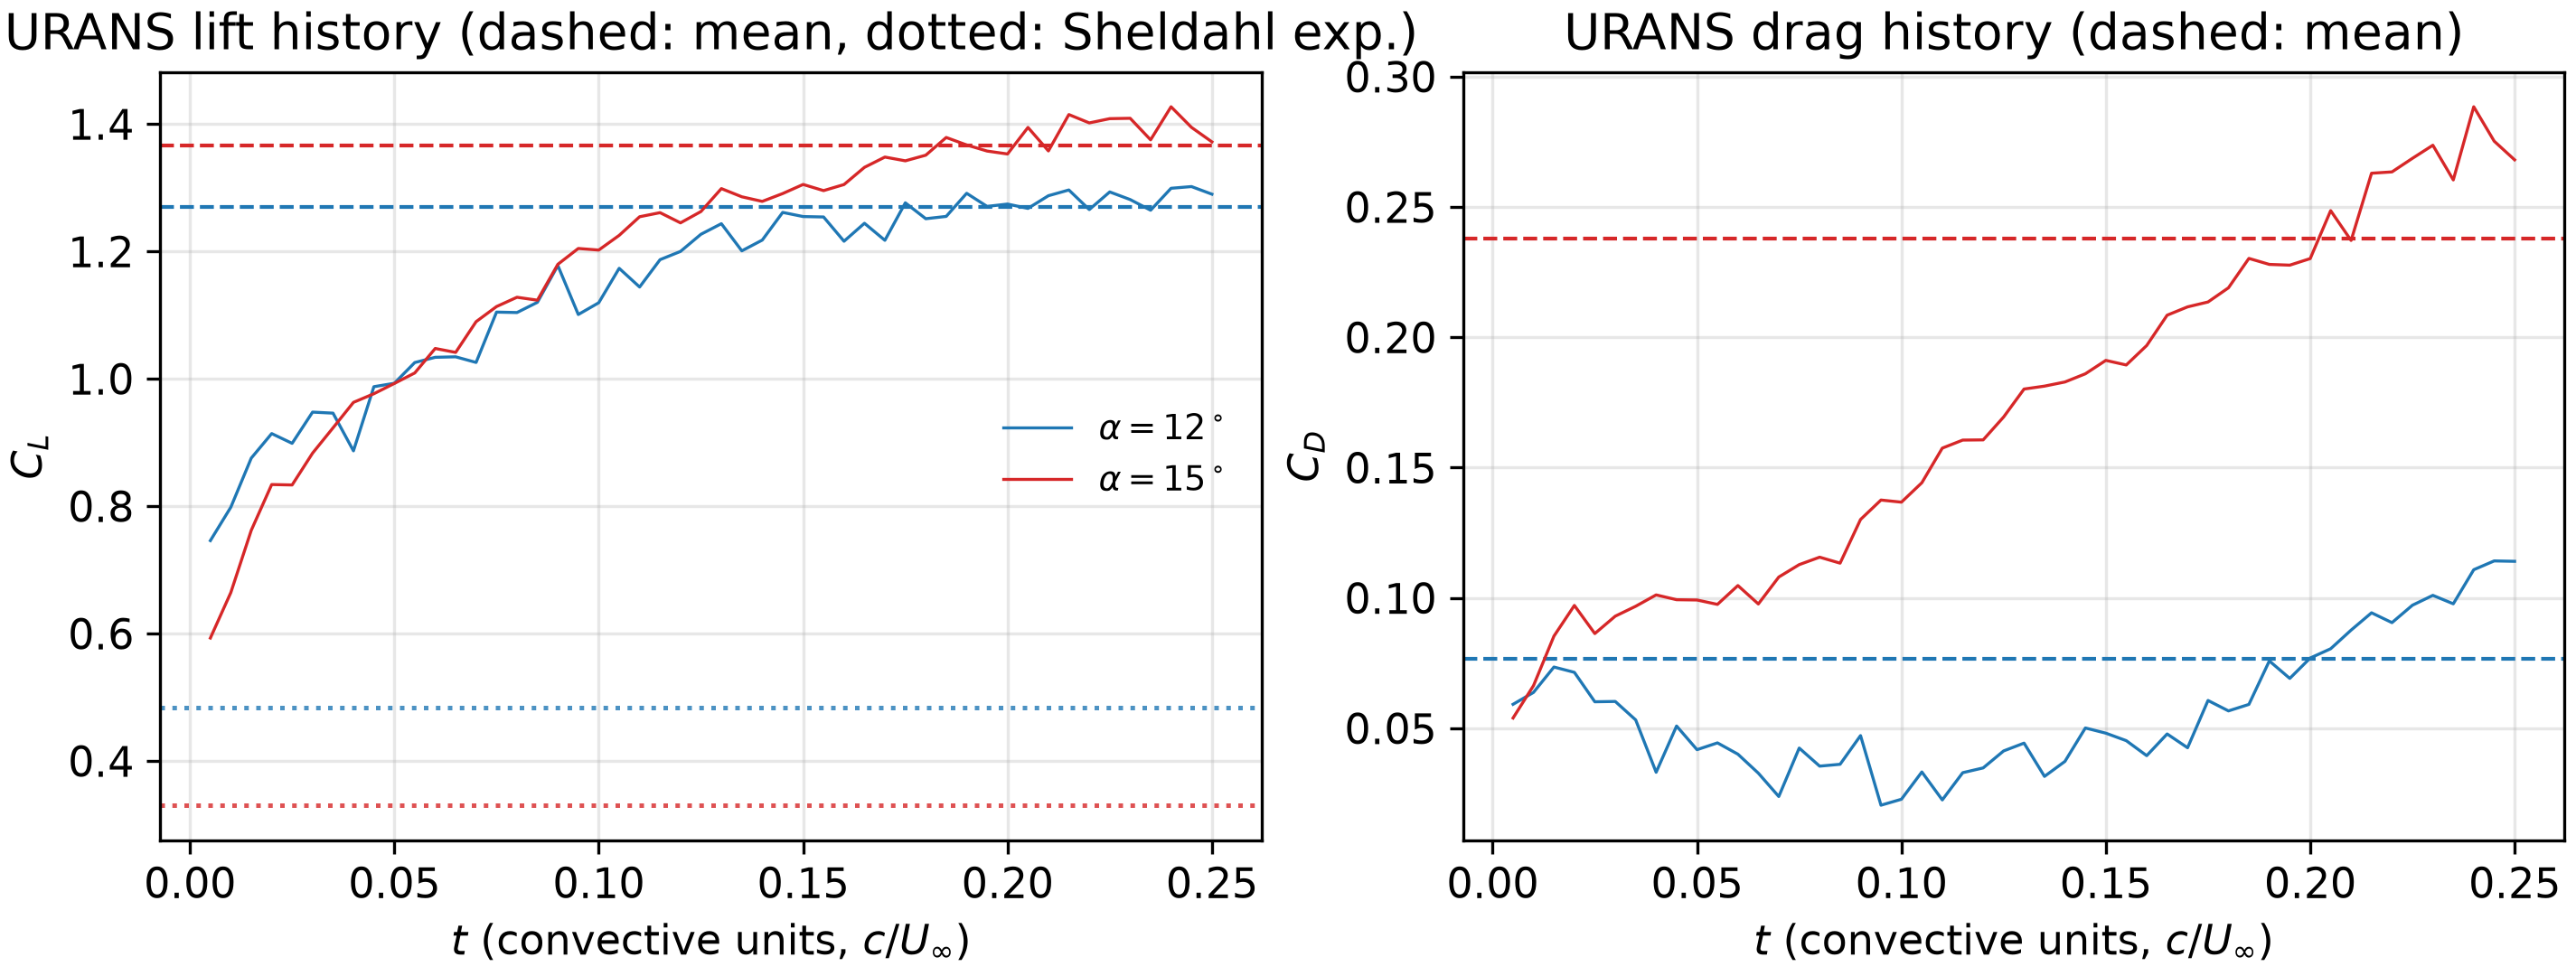
\includegraphics[width=0.72\textwidth]{figures/fig15_urans_history.png}
  \caption{URANS force histories versus convective time $t^*$ (one unit = one flow pass). Dashed: production-window means ($t^* = 0.81$--$2.4$); dotted: Reynolds-matched experimental values.}
  \label{fig:urans}
\end{figure}

\section{Conclusions}
\vspace{-0.4em}
For attached-flow drag and lift at matched Reynolds number, the transition closure is decisively better than the fully turbulent assumption, and the workflow is fully validated against code and experiment. At stall, however, steady 2D RANS is limited twice over: separation onset is grid-branch-dependent, and the converged steady state is not an attractor of the time-accurate system --- steady loads are a lower bound, not an equilibrium. Passive-device effects are out of scope for 2D RANS by construction. Scale-resolving 3D simulation with resolved transition remains the required next step and is listed as future work. Every artifact --- 125 cases, meshes, scripts 00--11, figures, and this report --- is released in the AERO-BLS repository for end-to-end reproduction.

\begin{thebibliography}{9}\small
\bibitem{langtry2009} R.~B. Langtry and F.~R. Menter, \emph{AIAA Journal} 47(12):2894--2906, 2009.
\bibitem{sheldahl1981} R.~E. Sheldahl and P.~C. Klimas, Sandia Report SAND80-2114, 1981.
\bibitem{abbott1959} I.~H. Abbott and A.~E. von Doenhoff, \emph{Theory of Wing Sections}, Dover, 1959.
\bibitem{ladson1988} C.~L. Ladson, NASA TM-4074, 1988.
\bibitem{gregory1970} N. Gregory and C.~L. O'Reilly, NASA R\&M 3726, 1970.
\bibitem{mccroskey1987} W.~J. McCroskey, NASA TM-100019, 1987.
\bibitem{spalart2000} P.~R. Spalart, \emph{Int. J. Heat Fluid Flow} 21(3):252--263, 2000.
\end{thebibliography}

\end{document}
